\clearpage
\subsection{Parte 2: Circuito RC in corrente impulsata - carica e scarica}
\label{sec:C3_P2-1}

\subsubsection{Cenni Teorici}

Per la seconda legge di Kirchhoff, l'equazione del circuito RC è:
$$ V_{Resistore} + V_{Condensatore} = V_{generatore} $$
Si ha che $ V_{Resistore} = V_R = RI$ e $ V_{Condensatore} = V_C = \frac{Q}{C} $, dunque:
$$ R \frac{\mathrm d Q }{\mathrm d t} + \frac{Q}{C} = V_{generatore} $$
%

\subsubsection*{Carica (da $0$ a $V_0$)}

Si ha $V_{generatore} = V_0$, e la condizione iniziale $Q(t=0) = 0 $ (poichè un istante prima il generatore è spento).\\
Usando il metodo della separazione delle variabili, e ponendo $\tau = CR $, si trova la soluzione:
$$ Q(t) = CV_0(1-e^{-\frac{t}{\tau}})$$
Da cui:
\[
  \begin{cases}
    V_R(t) = I(t) R = \frac{\mathrm d Q(t) }{\mathrm d t} = V_0e^{-\frac{t}{\tau}}\\
    V_C(t) = V_0 - V_R(t) = V_0(1-e^{-\frac{t}{\tau}})\\
  \end{cases}
\]



\subsubsection*{Scarica (da $V_0$ a $0$)}

Si ha $V_{generatore} = 0$, e la condizione iniziale $Q(t=0) =CV_0 $ (poiché un istante prima il generatore eroga $V_0$).\\
Come prima, usando il metodo della separazione delle variabili, e ponendo $\tau = CR $, si trova la soluzione:
$$ Q(t) = CV_0 e^{-\frac{t}{\tau}}$$
Da cui:
\[
  \begin{cases}
    V_R(t) = I(t) R = \frac{\mathrm d Q(t) }{\mathrm d t} = -V_0e^{-\frac{t}{\tau}}\\
    V_C(t) = - V_R(t) = V_0-e^{-\frac{t}{\tau}}\\
  \end{cases}
\]

\newpage
\subsubsection{Analisi dati}
Seguono qui i dati fittati con le equazioni appena ricavate.\\
%
% Grafico RC
%
    \begin{figure}[H]
    \centering
    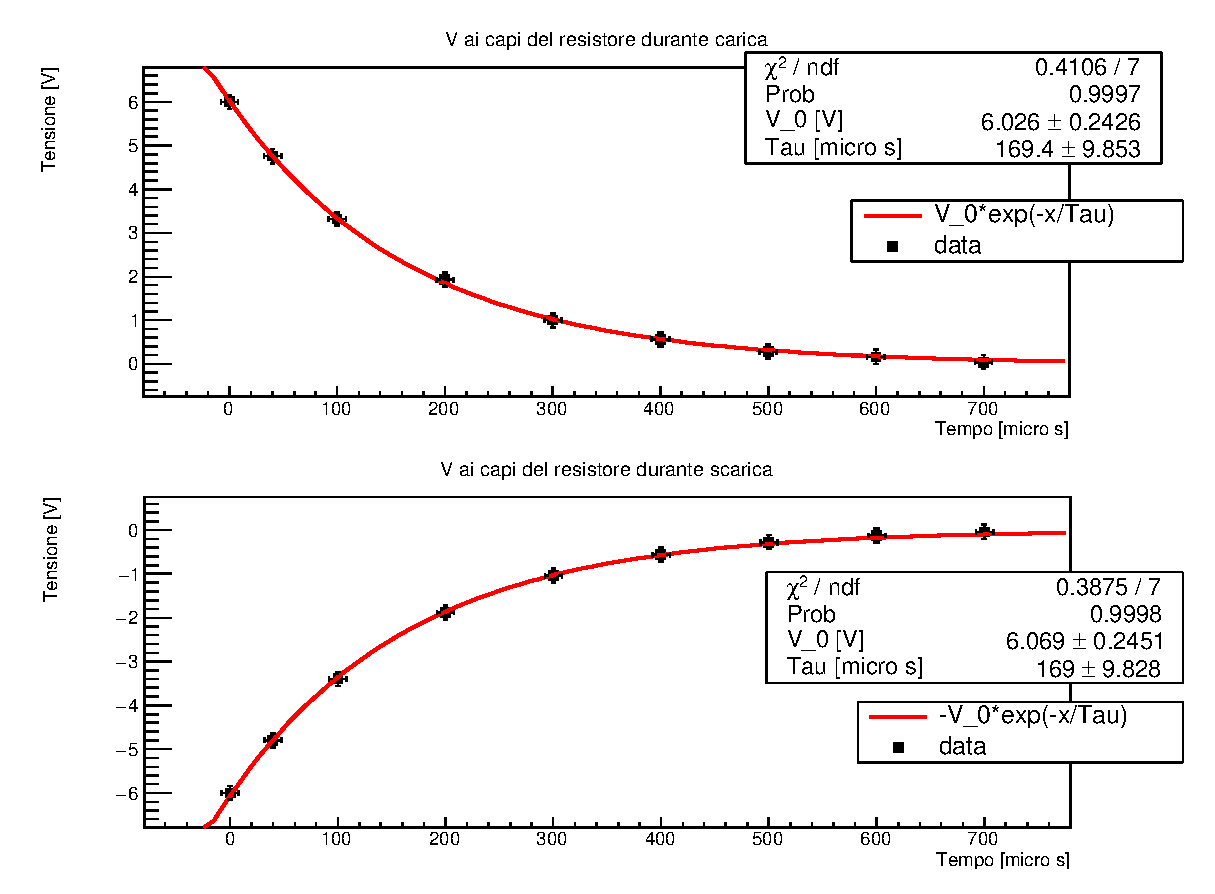
\includegraphics[scale=0.8]{Grafici/C3_P2_RC_impulsata_resistore.eps}
    %\caption{}
    \end{figure} 
%
    \begin{figure}[H]
    \centering
    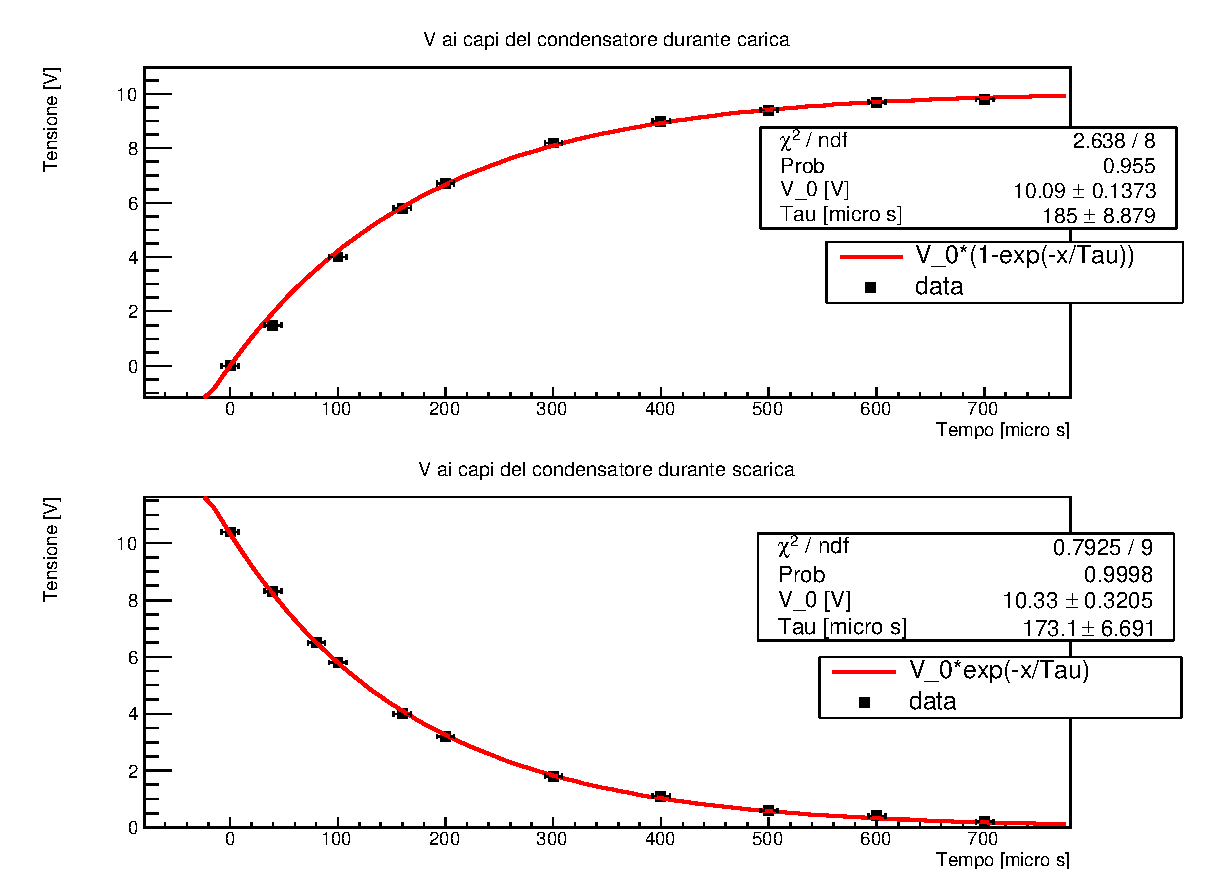
\includegraphics[scale=0.8]{Grafici/C3_P2_RC_impulsata_condensatore.eps}
    %\caption{}
    \end{figure} 
%
%
L'errore sulla tensione è stato stimato 0.16 V e quello per il tempo 8 µs (legati alla lettura dei valori con i cursori dell’oscilloscopio).\\
La resistenza usata è $14900 \pm 200$ Ohm (l'errore è stato calcolato come indicato sul manuale tecnico dello strumento).\\\\
%
%
Si ottiene il valore di $\tau$ con il suo errore calcolando la media pesata dei quattro valori ottenuti dai quattro fit.
%
Si ricava il valore della capacità $C$ e il suo errore, conoscendo la relazione $\tau = RC$ e utilizzando la formula di propagazione dell'errore.\\

Risultati ottenuti:
$$\tau = 174 \pm 4 \mu s $$
$$ C = 11.7 \pm 0.4  nF$$